\documentclass[11pt,norsk,a4paper]{article}
\usepackage[T1]{fontenc}
\usepackage[utf8]{inputenc}
\usepackage{babel}
\usepackage{amsmath}
\usepackage{amsfonts}
\usepackage{amsthm}
\usepackage{subfigure}
\usepackage{../MAT-INF1100-oppg}
\usepackage{xcolor}
\usepackage{tikz}
\usetikzlibrary{decorations.pathreplacing}
\usepackage[hidelinks]{hyperref}
%\usepackage{wrisym}
%\usepackage{lucidabr}
\textwidth=14cm \oddsidemargin=1cm \evensidemargin=0cm		% A4
%\newif\ifpdf
%\ifx\pdfoutput\undefined
%\pdffalse % we are not running PDFLaTeX
%\else
%\pdfoutput=1 % we are running PDFLaTeX
%\pdftrue
%\fi
%
%\ifpdf
%\usepackage[pdftex]{graphicx}
%\else
%\usepackage{graphicx}
%\fi

\usepackage{listings}

\lstdefinelanguage{matlab}
{
  morekeywords={if,else,end,for,while,do,def,break,return},
  sensitive=false,
  morecomment=[l]{//}
}
  
\lstset{language=matlab,
  backgroundcolor=\color[rgb]{.95,.95,.95},
  numbers=none,xleftmargin=10pt,
  numberstyle=\tiny,stepnumber=5,numbersep=5pt,
  stringstyle=\color{red},
  basicstyle=\ttfamily,
  keywordstyle=\color{blue},
  commentstyle=\color{green},
  basewidth=0.45em,
  showstringspaces=false,
  captionpos=b,
  frame=single
}

\title{Obligatorisk oppgave2 i MAT-INF 1100 høsten 2017}


\begin{document}
%\begin{flushright} \small 1.~november, 2017
%     \end{flushright}
%\vspace{10mm}

\begin{center}\huge MAT-INF 1100: Obligatorisk oppgave 2\\
     \vspace{5mm}
\Large  Innleveringsfrist: torsdag 8. november 2018 kl. 14:30
\end{center}

\section*{}
Obligatoriske oppgaver («obliger») er en sentral del av MAT-INF1100 og er utmerket trening i å besvare en matematisk oppgave.
Denne veiledningen er ment for å klargjøre noen krav vi som retter obligene stiller, både for å forenkle vår jobb i retteprosessen og for at dere skal slippe å måtte levere på nytt på grunn av formaliteter.

For å få godkjent en oblig bør man ha fått til om lag 2/3 av oppgavesettet og gitt alle deloppgavene et seriøst forsøk. 
Dersom det allikevel skulle være en oppgave du overhodet ikke får til, prøv å sette ord på hva du har tenkt og hvor det ikke lot seg løse.
Dersom man får «ikke godkjent» på en oblig og får et nytt forsøk vil det ha innleveringsfrist to uker etter første innlevering.  

\section{Krav til innlevering}

\begin{itemize}
	\item Besvarelsen skal leveres elektronisk via Devilry (\url{https://devilry.ifi.uio.no/}). Du velger selv om du skriver besvarelsen for hånd (og scanner besvarelsen) eller om du skriver løsningen direkte inn på datamaskin (f.eks. ved bruk av \LaTeX). Skannede ark må være godt lesbare. Godkjente filtyper: PDF

	\item Hoveddelen av besvarelsen skal leveres som én fil og i PDF-format. Det er lov å skanne inn håndskrevne ark så lenge disse er godt lesbare. 

	\item Besvarelsen skal inneholde navn, emne og oblignummer.

	\item Husk at andre skal lese og forstå din besvarelse! Besvarelsene bør derfor føres på en oversiktlig måte i den rekkefølgen de står oppgitt.

	\item Alle plott og figurer som er med på å besvare oppgaven må inkluderes (husk også riktige akser og enheter). Du bør også skrive kort hva hver figur viser, for eksempel:
	\textit{Figur 2: Plott av funksjonen $f(x) = x^2 -3$.}

	\item Kode kan leveres ved siden av besvarelsen, men \textbf{all diskusjon} og \textbf{all besvarelse} av oppgaven skal inn i hovedfila. 
	Det vil f.eks. si at du ikke kan levere et Python-skript som besvarelse på en oppgave hvor du blir bedt om å lage en algoritme. Det er viktig at programkoden du leverer inneholder et kjøreksempel, slik at det er lett å se hvilket resultat programmet gir. 

	\item Det oppmuntres til samarbeid om oppgavene, men du skal selv ha formulert og skrevet den besvarelsen som leveres inn, og den skal gjenspeile din forståelse av stoffet. Du kan bli bedt om å redegjøre muntlig for innholdet i din besvarelse.

	\item Besvarelsen bør inneholde diskusjon om resultatene dere kommer fram til. Eksempler på spørsmål man kan stille seg for å vite hva man skal kommentere er: \textit{Gir dette plottet noen mening?} \textit{Ser virkelig grafen til $f(x)$ slik ut?} \textit{Var dette resultatet som forventet?} \textit{Kan dette skyldes numeriske feil?} 
\end{itemize}

\noindent
Husk at de to obligatoriske oppgavene i MAT-INF 1100 begge må bestås for å kunne gå opp til endelig eksamen i emnet.

\paragraph{Søknad om utsettelse av innleveringsfrist}Hvis man blir syk eller av andre grunner trenger å søke om utsettelse av innleveringsfristen må du ta kontakt med studieadministrasjonen ved Matematisk institutt (7. et. Niels Henrik Abels hus, e-post: studieinfo@math.uio.no) i god tid før innleveringsfristen. 
For fullstendige retningslinjer for innlevering av obligatoriske oppgaver se
\begin{center}
uio.no/studier/admin/obligatoriske-aktiviteter/mn-math-oblig.html
\end{center}

\section{\LaTeX}

Vi oppmuntrer til bruk av \LaTeX. Dette er et slags programmeringsspråk for å skrive naturfaglige dokumenter som det kan være greit å lære seg først som sist.
Hjelp til \LaTeX{} kan du få omtrent overalt, fra utallige forum på verdensveven til gruppelærere over hele MatNat-fakultetet. 
Dersom du trenger hjelp til å komme i gang vil du finne \LaTeX-versjonen av denne teksten samme sted som du finner PDF-filen. Vi vil også legge ut en \LaTeX-mal med eksempler på hvordan inkludere kode og figurer som du kan bruke til å gjøre obligene i MAT-INF1100 om du vil. 

\newpage

\begin{oppgaver}
\oppgave Ved hjelp av en GPS har vi målt farten $v$ til et objekt som beveger seg. Målingene er gjort ved $N+1$ tidspunkter $(t_i)_{i=0}^N$ slik at resultatet er en følge av tall-par $(t_i,v_i)_{i=0}^N$ der $v_i$ angir farten ved tidspunktet $t_i$.

\begin{deloppgaver}
\oppgave Gi en algoritme for å beregne en tilnærming til objektets aksellerasjon $a(t)=v'(t)$ ut fra de beregnede verdiene $(t_i,v_i)$ av farten.

\oppgave Gi en algoritme for å beregne en tilnærming til objektets avstand $s(t)$ fra startpunktet ut fra de beregnede verdiene når $v(t)=s'(t)$ og $s(t_0)=0$.

\oppgave Fila 
\begin{center}
%\small
\url{http://www.uio.no/studier/emner/matnat/math/MAT-INF1100/h18/obliger/running.txt} 
\end{center}
er en logfil fra en løpetur, der vi på hver linje finner kommaseparerte tid/fart-verdier. Du har lært at du kan lese inn verdiene fra denne fila i to
vektorer {\tt t} og {\tt v} ved hjelp av følgende kode:
\begin{lstlisting}
t = []
v = []
infile = open('running.txt','r')
for line in infile:
    tnext, vnext = line.strip().split(',')
    t.append(float(tnext))
    v.append(float(vnext))
infile.close()
\end{lstlisting}
Last ned fila {\tt running.txt} og kjør denne koden, og bruk algoritmene fra a) og b) til å lage to plott: Ett der du plotter objektets akselerasjon mot tid, og ett der du plotter
objektets avstand fra startpunktet mot tid.
\end{deloppgaver}





\oppgave 
Vi betrakter en pendel som ved tiden $t$ har et utslag på $\theta(t)$ radianer (se Figur \ref{fig:pendel}). Ved hjelp av Newtons 2.~lov og litt vektorregning, kan vi utlede differensialligningen
\begin{equation}\label{eq:pendel}
\frac{d^2\theta}{dt^2}(t) = -\frac{g}{L}\sin(\theta(t))
\end{equation}
der $g \approx 9.81 \frac{m}{s^2}$ er gravitasjonsaksellerasjonen og $L$ er lengden til pendelen. Pendelligningen \eqref{eq:pendel} er et eksempel på en enkel differensialligning som ikke har en løsning som uttrykkes ved enkel formel. I denne oppgaven skal vi se på to måter å tilnærme løsningen på: \emph{Linearisering} og \emph{numerisk simulering}.
\begin{figure}
\centering
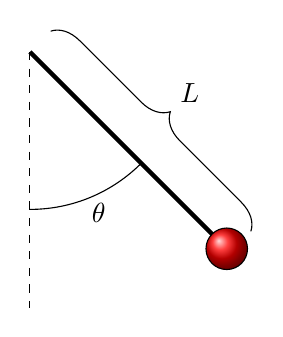
\begin{tikzpicture}[scale=2.5]
\draw[ultra thick] (0,0) -- (1,-1);
\draw[decorate,decoration={brace,amplitude=10pt},xshift=3pt,yshift=3pt] (0,0) -- (1.02,-1.02) node[midway,xshift=14pt,yshift=14pt]{$L$};
\draw[dashed] (0,0) -- (0,-1.3);
\draw[ball color=red] (1,-1) circle (3pt);
\begin{scope}
	\clip (0,0) -- (1,-1) -- (0,-1);
	\draw (0,0) circle (0.8);
\end{scope}
\draw (0.35,-0.82) node{$\theta$};
\end{tikzpicture}
\caption{En pendel består av en stang med et tung objekt i den ene enden, og som dreier om et punkt i den andre enden. Vi antar at stangen er helt stiv, er tilnærmet masseløs, og har lengde $L$.}
\label{fig:pendel}
\end{figure}

\begin{deloppgaver}
\oppgave
Hastigheten til pendelvekten er gitt ved $v(t) = L\frac{d\theta}{dt}(t)$. Forklar hvordan vi kan gjøre om den \emph{annenordens} differensialligningen \eqref{eq:pendel} til \emph{systemet av førsteordens} differensialligninger
\begin{equation}\label{eq:pendelsys}
\begin{split}
\frac{dv}{dt} &= -g\sin(\theta), \\[2pt]
\frac{d\theta}{dt} &= \frac{1}{L}v.
\end{split}
\end{equation}
Motsatt, hvordan finner du løsningen av \eqref{eq:pendel} om du kjenner løsningen av  \eqref{eq:pendelsys}?

\oppgave
Forklar hvorfor det \emph{lineære} systemet
\begin{equation}\label{eq:pendelsyslin}
\begin{split}
\frac{dv}{dt} &= -g\theta ,\\[2pt]
\frac{d\theta}{dt} &= \frac{v}{L}
\end{split}
\end{equation}
gir en god tilnærming til løsningen av det \emph{ikkelineære} systemet \eqref{eq:pendelsys} når utslaget til pendelen er lite. Finn løsningen av \eqref{eq:pendelsyslin} gitt startbetingelser $\theta(0)=\theta_0$, $v(0)=v_0$.

\noindent
\textit{Hint: For å løse \eqref{eq:pendelsyslin}, skriv om ligningen til en annenordens differensialligning ved å derivere ligningen for $\theta$.}

\oppgave
For et lite tall $h>0$ lar vi $t_k = hk$ for $k=0,1,\dots,N$, og vi lar $\theta_k, v_k$ være tilnærminger til $\theta(t_k), v(t_k)$. Eulers metode for \eqref{eq:pendelsyslin} er da
\begin{equation}\label{eq:eulerpendellin}
\begin{split}
v_{k+1} &= v_k - gh\theta_k, \\
\theta_{k+1} &= \theta_k + h\frac{v_k}{L},
\end{split}
\end{equation}
for $k=0$, 1, \dots, $N-1$.
Skriv en Python-funksjon \verb|lin_pendel_euler| som med funksjonskallet 
\begin{verbatim}
v, theta = lin_pendel_euler(v0, theta0, g, L, N, h);
\end{verbatim}
bruker Eulers metode for å beregne $v$ og $\theta$ gitt startbetingelser $v_0=\texttt{v0}, \theta_0=\texttt{theta0}$. Returverdiene \texttt{v} og \texttt{theta} skal være Python-lister av lengde $N+1$ og inneholde verdiene $\texttt{v[0]}=v_0, \texttt{v[1]}=v_1, \dots, \texttt{v[N]}=v_N$, og tilsvarende for \texttt{theta}.

\oppgave
Plott den numeriske løsningen for vinkelutslaget som en funksjon av tid sammen med den eksakte løsningen du fant i b). Kommenter forskjellene. Bruk verdiene $g=9.81$, $L=1$, $v_0=0$, $\theta_0=\frac{\pi}{2}$ og $h = T/N$, der $T=4$. Bruk først $N=2^{5}$ antall steglengder og deretter $N=2^{10}$.

\oppgave
For å beregne feilen i Eulers metode definerer vi 
\[
\epsilon(h) = |\theta_N-\theta(t_N)|,
\]
der $\theta_N$ er beregnet med Eulers metode \eqref{eq:eulerpendellin} med steglengde $h$, og $\theta(t)$ er løsningen du fant i b). (Vi ser bort fra feilen i $v$ her.) Beregn feilen $\epsilon(h)$ med verdiene $h=T/N$, der $N=2^{4},2^{5},\dots,2^{10}$. Bruk ellers de samme verdiene som i oppgave d). Oppgi feilene $\epsilon(h)$ i en tabell.

\oppgave
Vi sier at en numerisk metode er av orden $p$ dersom det finnes en konstant $C>0$ slik at $\epsilon(h) \leq Ch^p$ for små verdier av $h$. Vi kan finne tallet $p$ \emph{eksperimentelt} som følger: Anta at $\epsilon(h)=Ch^p$ for verdier av $C$ og $p$ (som vi ikke kjenner). Velg to forskjellige verdier $h=h_1,h_2$. Da er $\epsilon(h_1)/\epsilon(h_2) = (Ch_1^p)/(Ch_2^p) = (h_1/h_2)^p$. Løser vi for $p$, får vi
\[
p = \frac{\log\big(\epsilon(h_1)/\epsilon(h_2)\big)}{\log(h_1/h_2)}.
\]
Bruk tallene du fant i oppgave e) til å estimere konvergensraten $p$ for verdiene $h_1=T/N$ og $h_2=h_1/2$, der $N=2^{4},2^5\dots,2^{9}$. Oppgi estimatene for $p$ i en tabell. Hva tror du konvergensraten til Eulers metode er?

\oppgave
Dersom utslaget til pendelen er stort, vil løsningen av det lineariserte systemet \eqref{eq:pendelsyslin} raskt avvike fra løsningen av den opprinnelige ligningen \eqref{eq:pendelsys}. Skriv en Python-funksjon \verb|pendel_euler| som med funksjonskallet 
\begin{verbatim}
v, theta = pendel_euler(v0, theta0, g, L, N, h);
\end{verbatim}
bruker Eulers metode for å løse \eqref{eq:pendelsys}. Plott $\theta$ som en funksjon av tid fram til tiden $T=4$. Bruk en steglengde $h=T/N$, der $N=2^{10}$, og bruk ellers de samme verdiene som i oppgave d). Inkluder de to løsningene fra b) og c) i plottet. Kommenter forskjellene.

\oppgave
\emph{(Hvis du har tid)} \\
Systemet \eqref{eq:pendelsys} er et \emph{hamiltonsk system}, som kjennetegnes bl.a.~ved at det finnes en funksjon $H(v,\theta)$, \emph{hamiltonfunksjonen}, som er slik at $H(v(t),\theta(t))$ er konstant over tid. I dette tilfellet er $H(v,\theta)=-g\cos(\theta)+v^2/(2L)$, som kan tolkes som total (potensiell + kinetisk) energi for pendelen.
\begin{enumerate}
\oppgave Gjenta oppgave g), men med $T=50$. (Nå trenger du ikke plotte løsningene av det lineære systemet.) Hvordan tolker du plottet? Er energien til pendelen bevart i den numeriske løsningen? Hva skjer når du velger en større $N$?
\oppgave Eulers metode har en tendens til å tilføre energi til hamiltonske systemer. Skriv en Python-funksjon \verb|pendel_symp_euler| som implementerer den \emph{symplektiske Euler-metoden}\footnote{Symplektiske metoder er laget for å bevare hamiltonfunksjonen langt mer nøyaktig enn andre metoder. Disse metodene er svært viktige for å simulere hamiltonske systemer slik som planetbaner og partikler i partikkelakselleratorer.}
\begin{equation}\label{eq:sympeulerpendellin}
\begin{split}
v_{k+1} &= v_k - gh\sin(\theta_k) \\
\theta_{k+1} &= \theta_k + h\frac{v_{k+1}}{L}.
\end{split}
\end{equation}
Gjenta oppgave g) med denne metoden, men med $T=50$ og med $T=500$. Ser den numeriske løsningen riktigere ut med denne metoden?
\end{enumerate}
\end{deloppgaver}





\vspace{1cm}
\centerline{\em Lykke til!}

\end{oppgaver}




\end{document}




